\chapter{Anforderungserhebung}
In diesem Kapitel werden zwei Nutzerrollen aus dem Bereich des Netzwerkmanagements und der Netzwerksicherheit und ihre Arbeitsprozesse vorgestellt. Dabei wird insbesondere auf die Bedürfnisse der Rollen eingegangen und analysiert, wie diese Bedürfnisse dank neuer Software besser erfüllt werden können. Hieraus ergeben sich Anforderungen für die Konzeption und Implementierung der besagten Software.

\section{Nutzer}
%Thesis Fragestellung aufgegriffen
    Um die Frage beantworten zu können, ob es möglich ist, die übertragenen Daten der intelligenten Geräte herstellerübergreifend zu überwachen, ist es nötig, Zugriff auf die eingehenden sowie ausgehenden Daten der Geräte zu erhalten. In diesen Daten, welche vom \ac{IoT}-Gerät zum Broker und andersherum geschickt werden, befinden sich möglicherweise personenbezogene Daten sowie Hinweise auf mögliche Schwachstellen.
    Die nächste Herausforderung besteht darin, die gesammelten Daten einem Nutzer in einer aufbereiteten Ansicht zugänglich zu machen und die direkte Interaktion mit den Daten zu ermöglichen.

    Aus diesem Überlegung ergeben sich zwei wichtige Nutzerrollen: Netzwerk- und Systemadministratoren und Security-Auditoren.
    
%=====================================================================%    
%Wer? Nutzerrolle: Admin (monitoring)
%=====================================================================%    
    \subsubsection{Netzwerk- und Systemadministratoren} \label{NetzwerkUndSystemadmin}
    Auf der einen Seite existiert der System- und Netzwerkadministrator, welcher versucht, Probleme in der Kommunikation zu finden und zu lösen oder eventuelle Anomalien darin zu erkennen.
%Aufgabenbereiche Motivation
    Nach Burgess \cite{burgess2004principles} zählen zu den Aufgabenbereichen von Netzwerk- und Systemadministratoren unter anderem:
    \begin{itemize}
        \item \glqq Diagnostics, fault and change management\grqq{}
        
        Eine Aufgabe ist, Systeme für das eigene Unternehmen oder Kunden bereitzustellen und Störungen darin zu beheben. Um bei Problemen herausfinden zu können, wo diese entstanden sind und wie sie schnell behoben werden können, ist es hilfreich, die Kommunikation im Netzwerk zu beobachten. Zum Beispiel kann erkannt werden, ob \ac{TCP}-Pakete überhaupt am Ziel ankommen oder schon auf dem Übertragungsweg verloren gehen. Abhängig davon, kann das Problem weiter eingeschränkt und schließlich lokalisiert werden.
        
        \item \glqq Configuration and maintenance\grqq{}
        
        Für eine korrekte Konfiguration der Systeme ist es notwendig, die Kommunikation nachvollziehen zu können. Dazu muss ein Verständnis der genutzten Technologien vorhanden sein. Außerdem sollte bekannt sein, welche Art von Daten übertragen werden.
        
        %Performance regarding bottlenect.
        Dank der Informationen aus den aufgezeichneten Datenpaketen, wie deren Größe und dem Zeitstempel, können anhand von statistischer Analyse Rückschlüsse auf die Netzwerkbelastung gezogen werden.
        
        \item \glqq Application-level services\grqq{}
        
        %Reverse Proxies und DNS
        Hier müssen Administratoren verschiedene Applikationen (beispielsweise \ac{DNS}-Server oder Proxys) konfigurieren und Anwendungen miteinander verbinden, um neue Systeme in bestehende Systemlandschaften zu integrieren.
        
        \item \glqq Network-level services\grqq{}
        
        Auch können verschiedene Protokolle miteinander verbunden werden.
        %TODO: bisschen mehr..
        
    \end{itemize}

% Ziel
    Das Ziel eines Netzwerkadministrators ist somit die Identifikation von Störquellen sowie das Sicherstellen der Verfügbarkeit aller geschäftskritischen Dienste (\emph{high availability}) \cite{burgess2004principles}. Dies ist eine wichtige Voraussetzung für hohe Kundenzufriedenheit.
    
%was gibt es bereits (Wireshark) was kann die Software besser/kann nur die Software
    Wie bereits erwähnt, gibt es für die einzelnen Phasen verschiedene Werkzeuge, die sich in der Praxis etabliert haben und Anwender in ihrer Arbeit unterstützen.
    %https://proquestcombo.safaribooksonline.com/9781492020356
    Wireshark, eine Anwendung zum Überwachen und Aufzeichnen von Netzwerkverkehr, stellt ein wichtige Komponente der zu konzipierenden Software dar \cite{SandersChris2017Ppa}. Ein wichtiger Unterschied besteht jedoch darin, dass in dem Konzept der Arbeit zusätzlich direkt in die Kommunikation eingegriffen werden muss. Das bedeutet, dass Nachrichten verändert, verworfen oder erneut gesendet werden sollen, was durch ein reines Monitoring-Tool nicht möglich ist.
    
% Was müsste die eigene Software verbessern
    %Log Messages
    Der Nutzer soll, wenn er mit diesem Programm arbeitet, den Proxy in den Modus \glqq intercept\grqq{} oder \glqq none intercept\grqq{} stellen können, um Inhalte spezieller Clients einzeln und gezielt prüfen zu können, ohne Daten anderer Geräte im Netzwerk zu erhalten.
    %View Messages
    Weiterhin möchte der Nutzer, dass die Nachrichten, welche durch den \glqq intercept\grqq{}-Modus abgefangen wurden, aufgelistet und angezeigt werden.
    %View ClientInfos
    Für den Fall, dass etwas nicht ordnungsgemäß funktioniert oder fehlerhaft konfiguriert wurde, ist es ebenfalls relevant, die Verbindungsdaten der einzelnen Proxy-Clients, die eine Verknüpfung zu dem zu untersuchenden \acs{IoT}-Gerät haben, einsehen zu können.
    
%=====================================================================%
%wer? Nutzerrolle: Security Auditor
%=====================================================================%
% Motivation
\subsubsection{Security-Auditor}
    Auf der anderen Seite existiert der Security-Auditor (auch "Penetration-Tester") welcher versucht, Schwachstellen in Kommunikation, Geräten oder Endpunkten zu identifizieren.
% Ziel
    Dies befähigt den Hersteller, von dem der Tester beauftragt wird, seine Produkte im Rahmen der Qualitätssicherung vor ihrer Veröffentlichung zu testen, um Fehler zu erkennen, diese beheben zu können und somit potentielle Probleme zu vermeiden. Das ist nicht nur für Vertrauen innerhalb der Branche wichtig, sondern darüber hinaus in bestimmten Bereichen (z.B. kritischen Infrastrukturen) sogar gesetzlich vorgeschrieben.
    Zusätzlich bestätigt es, dass der Dienst eines Unternehmens gute und effiziente Sicherheitsmechanismen korrekt implementiert hat, um die Kundendaten vor Gefährdungen der Vertraulichkeit, Integrität oder Verfügbarkeit zu schützen.
    
    Ein weiterer wichtiger Untersuchungsgegenstand sind personen- und unternehmensbezogene Daten. Der Schutz dieser hat aufgrund von datenschutzrechtlichen Bestimmungen eine besonders hohe Priorität. Dies wird in Form von manueller oder regelbasierter Inspektion der Übertragung überprüft.
    
%Was für Arbeitsabläufe
    
    %wie: Wie hilft die Software dabei das Ziel zu erreichen
    Die in dieser Arbeit zu konzipierende Software soll den Tester mithilfe von passivem Scannen und Abfangen der Kommunikation in Kapitel \ref{IntelligenceGathering} Punkt 2 (\emph{Intelligence Gathering}) und durch Manipulieren sowie erneutes Senden der Nachrichten in Schritt 5 (\emph{Exploitation}) unterstützen.
    
    %was gibt es bereits (Wireshark) was kann die Software besser/kann nur die Software
    Wie in Kapitel \ref{NetzwerkUndSystemadmin} beschrieben, kann Wireshark zur Informationsbeschaffung verwendet werden.
    Da von Wireshark viele verschiedene Protokolle unterstützt und auch sehr detaillierte Informationen angezeigt werden, passiert es schnell, dass durch die große Menge wichtige Bestandteile untergehen (auch \emph{visual clutter} genannt) oder nur mit Aufwand gefunden werden.
    
    Burp Suite von PortSwigger bietet wie Wireshark eine Proxy-Komponente und kann somit nicht nur, wie in diesem Tool geplant, die Nachrichten protokollieren bzw. überwachen, sondern auch in die Kommunikation eingreifen. Der große Unterschied besteht darin, dass Burp Suite ausschließlich für HTTP/S und (Sec)Websocket Kommunikation zu verwenden ist und keinerlei Unterstützung für das \ac{MQTT}-Protokoll bietet. Ähnliche Abläufe und eine strukturierte Darstellung, wie in Burp Suite, wären von Vorteil, um die Einarbeitungszeit gering zu halten und die Akzeptanz bei den Nutzern zu stärken.

\section{Abgeleitete Anforderungen}
    Im Folgenden werden Use-Cases aus den obigen Nutzerbeschreibungen extrahiert und beschrieben.
    %Aus Beschreibung ergeben sich Use-Cases
    \subsection{Use-Cases}
    \begin{figure}[h]%h=direkt danach t=top b=bottom
        \centering
        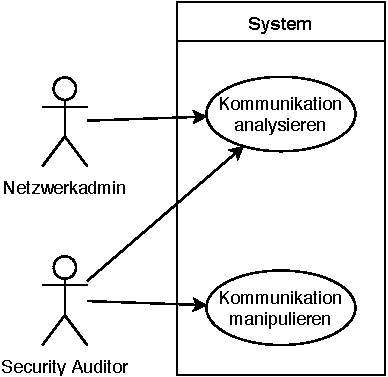
\includegraphics[width=7cm]{tex/bilder/3_anforderungen/Use-Case.pdf}
        \captionof{figure}{Use-Case-Diagramm}
        \label{fig:use-case}
    \end{figure}
    
    Zum ersten Use-Case \emph{Kommunikation analysieren}:
    	Der Nutzer möchte die Nachrichten der \ac{MQTT}-Kommunikation analysieren.
    	Darüber hinaus ist es notwendig, das Abfangen der Pakete pro Gerät einstellen zu können, um nur die gewünschte Kommunikation mitzuschneiden und somit eine selektive Analyse zu ermöglichen.
    	Um dies zu bewerkstelligen, ist es notwendig, die abgefangen Daten nach deren Inhalten zu filtern.
    	
    Zu \emph{Kommunikation manipulieren}:
        Über eine Manipulation der Kommunikation spricht man, sobald existierende Pakete verändert oder neue versendet werden. Dadurch, kann die Kommunikation über verschiedene Aktionen manipuliert werden. \glqq Payload ändern\grqq{}, \glqq Nachricht senden\grqq{}, \glqq Nachricht kopieren\grqq{}, \glqq Nachricht ändern\grqq{}, \glqq Nachrichten speichern\grqq{} und \glqq Nachricht verwerfen\grqq{} sind die in dieser Arbeit betrachteten Elemente.
    	Der Nutzer möchte auf verschiedene Weisen die Kommunikation zwischen zwei Kommunikationspartnern über ein drittes System verändern können.
    	Durch Manipulation der übertragenen Daten einzelner Nachrichten ist es dem Nutzer möglich, die Kommunikation zu verändern.
    	Anhand von selbsterstellten Paketen, welche im Namen der Kommunikationspartner erstellt werden, sollen vom Nutzer gewünschte Informationen übertragen werden.
    	Um die repetitive Arbeit der Nachrichtenerstellung zu beschleunigen, kann eine abgefangene Nachricht kopiert werden.
    	Diese Änderungen sollen anschließend gespeichert werden können, um veränderte Pakete zu einem späteren Zeitpunkt versenden oder erneut verändern zu können.
    	Für den Fall, dass übertragene Nachrichten Inhalte beinhalten, welche nicht ankommen dürfen oder nicht den gewünschten Inhalt haben, soll der Nutzer diese verwerfen und somit nicht dem Zielgerät zustellen.

    %Tabelle mit Funktionale Anforderungen
    \subsection{Formale Anforderungen} \label{FormaleAnforderungen}
    Anhand der Use-Cases lassen sich folgende formale Anforderungen ableiten (siehe Tabelle \ref{tab:functional_requirements}).
    Dabei ist zu beachten, dass diese Anforderungen dadurch, dass es sich um ein abstraktes Konzept handelt, unspezifisch und ausschließlich funktional sind.
    \begin{table}[h]
        \centering
        \begin{tabular}{c|c}
            \hline
            $Nr.$ & $Name$ \\ \hline
            %Nachricht abfangen vllt auch ein Feature was nennenswert ist oder wird es m it Nr.3 abgedeckt???
            1 & Nachrichten anzeigen \\ \hline
            2 & Nachrichten filtern \\ \hline
            3 & Abfangen umschalten \\ \hline
            4 & Nachricht manipulieren \\ \hline
            5 & Nachricht senden \\ \hline
            6 & Nachricht verwerfen \\ \hline
        \end{tabular}
        \caption{Funktionale Anforderungen}
        \label{tab:functional_requirements}
    \end{table}
    
        \subsubsection{1. Nachrichten anzeigen}
        Das System ermöglicht die Anzeige von Nachrichten einer \ac{MQTT}-Kommunikation.
        Dabei werden diese in einer chronologischen Reihenfolge dargestellt und stellen relevante Informationen wie Topic, Payload, Quality of Service und Zeitpunkt der Übertragung zur Verfügung.
        In dieser Arbeit werden jedoch nicht alle eingehenden, sondern nur aktiv abgefangene Nachrichten betrachtet, da diese die höchste Priorität besitzen.
        
        \subsubsection{2. Nachrichten filtern}
        Die Software muss angezeigte Nachrichten nach deren Attributen filtern können. Diese sind unter anderem \glqq Payload\grqq{}, \glqq Client\grqq{} und \glqq Quality of Service\grqq{}.
        
        \subsubsection{3. Abfangen umschalten}
        Dem Nutzer muss die Möglichkeit gegeben werden, das Abfangen der  Kommunikation der \ac{IoT}-Geräte zu aktivieren oder zu deaktivieren.
        Dabei werden die Pakete in die Warteschlange eingetragen, und dürfen nicht an den Kommunikationspartner weitergeleitet werden.
        Dies muss durch den Nutzer, für jedes verbundene Gerät, konfigurierbar sein.
        
        \subsubsection{4. Nachricht manipulieren}
        Der Nutzer muss den Inhalt der aufgezeichneten Nachrichten manipuliert können. Vorrangig muss der übertragene Nachrichteninhalt auf einen gewünschten Wert abgeändert werden können.
        
        \subsubsection{5. Nachricht senden}
        Es muss garantiert werden, dass selbst erstellte Nachrichten gesendet werden können.
        Das Senden beinhaltet nicht nur die Übertragung dieser, sondern umfasst auch das erneute Senden (auch \emph{replay attack} genannt) von bereits übertragenen Nachrichten. Die Inhalte werden in diesem Fall nicht verändert, sondern wie erfasst erneut versendet.
        
        \subsubsection{6. Nachricht verwerfen}
        Das System muss es dem Nutzer ermöglichen, abgefangene Nachrichten zu verwerfen.
        Dies bedeutet, dass gesendete Inhalte nicht an den gewünschten Kommunikationspartner weitergeleitet werden. Stattdessen werden sie, nachdem sie abgefangen wurden, aus der Kommunikation entfernt.
        Die ausgewählten Nachrichten werden somit auch in der Oberfläche nicht weiter angezeigt.
        
\subsubsection{Zusammenfassung}
    In diesem Kapitel wurden die Tätigkeiten der vorgestellten Nutzerrollen beschrieben, ihre Arbeitsprozesse dargestellt und noch verbesserungswürdige Prozessschritte identifiziert. Anhand dieser Verbesserungspotenziale wurden anschließend funktionale Anforderungen definiert, welche die Grundlage für das Konzept bilden.